\documentclass{article}
\usepackage[utf8]{inputenc}
\usepackage{titling}
\usepackage{enumitem}
\usepackage{graphicx}
\usepackage{xcolor}
\usepackage[colorlinks=true,linkcolor=darkgray, urlcolor =gray]{hyperref}
\usepackage[spanish]{babel}
\DeclareUnicodeCharacter{301}{~}
\usepackage{url}


\title{Práctica 4. Razonamiento e inferencias con GENIE}
\author{Cristina Díaz García}
\date{Abril 2019}

\renewcommand\maketitlehooka{\null\mbox{}\vfill}
\renewcommand\maketitlehookd{\vfill\null}


\begin{document}

\addcontentsline{toc}{section}{Índice general}

\begin{titlingpage}
\maketitle
\end{titlingpage}

\newpage

\tableofcontents

\newpage

\section{Enunciado}

\textbf{\underline{Tarea:}} Resuelve los siguientes ejercicios con ayuda de GENIE

\textbf{\underline{Entrega:}} Documento pdf con la información que se pide en cada ejercicio

\section{\textbf{Ejercicio 1}}

Implementa ejemplos (los de los apuntes o inventados por ti) de todas las posibles
estructuras de redes con tres nodos (cola-con-cola, cabeza-con-cabeza, cabeza-con-cola). En el caso de la estructura cabeza-con-cabeza, implementa un modelo AND y un modelo OR. Realiza
pruebas de inferencia con las estructuras y comprueba que los resultados obtenidos son acordes con las relaciones de independencia que hemos estudiado en clase para dichos modelos. En el caso de la estructura cabeza-con-cabeza, comprueba que en el modelo OR se da el efecto
explaning-away, y estudia qué ocurre en el modelo AND. Escribe un pequeño informe con
capturas de pantalla de las redes y los resultados y conclusiones que hayas obtenido.

\subsection{\textbf{Cola-con-cola}}

\textbf{Modelo inicial}

\begin{center}
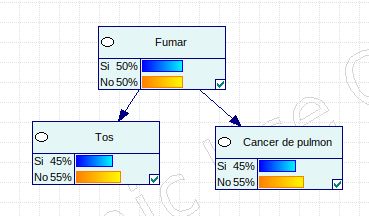
\includegraphics[scale=0.5]{1a1.png}
\end{center}

\textbf{Instanciamos un nodo hijo}

\begin{center}
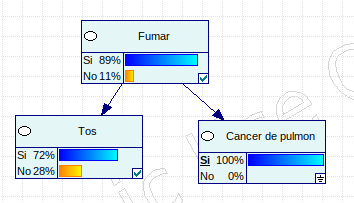
\includegraphics[scale=0.5]{1a2.png}
\end{center}

Comprobamos que este valor sí afecta al otro nodo hijo.

\newpage

\textbf{Instanciamos el nodo padre}

\begin{center}
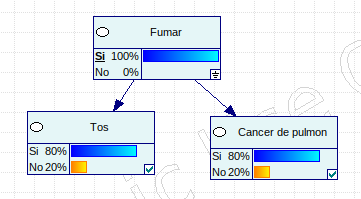
\includegraphics[scale=0.5]{1a3.png}
\end{center}

\begin{center}
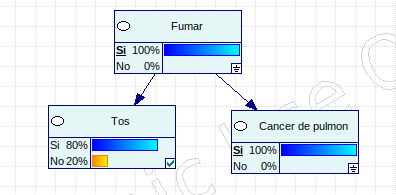
\includegraphics[scale=0.5]{1a4.png}
\end{center}

Podemos ver que el valor de un nodo hijo no afecta al otro, ya que el valor lo ha tomado por la probabilidad del padre.

\subsection{\textbf{Cabeza-con-cabeza}}

\textbf{Modelo AND inicial}

\begin{center}
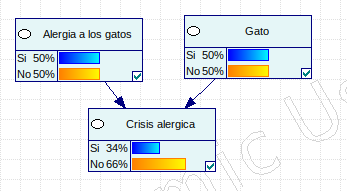
\includegraphics[scale=0.5]{AND1.png}
\end{center}

\textbf{Modificamos uno de los nodos padres y el nodo hijo}

\begin{center}
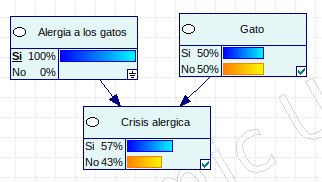
\includegraphics[scale=0.5]{AND2.png}
\end{center}

\begin{center}
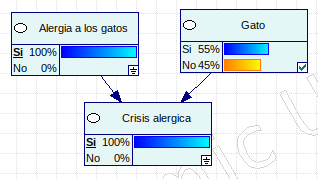
\includegraphics[scale=0.5]{AND3.png}
\end{center}

Como se comprueba, el valor del otro nodo padre, varía al cambiar tamién el valor del nodo hijo, pero no por el cambio del primer nodo padre.\\

\textbf{Modificamos el nodo hijo y uno de los nodos padres}

\begin{center}
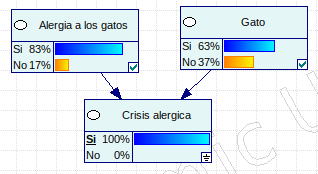
\includegraphics[scale=0.5]{AND4.png}
\end{center}

\begin{center}
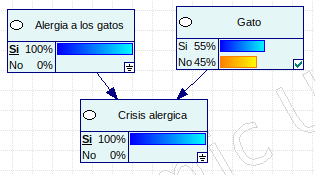
\includegraphics[scale=0.5]{AND5.png}
\end{center}

Como se comprueba, el valor del otro nodo padre, varía al cambiar tamién el valor del nodo padre.\\

\textbf{Modelo OR inicial}

\begin{center}
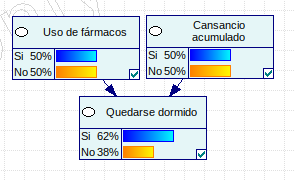
\includegraphics[scale=0.5]{OR1.png}
\end{center}

\newpage

\textbf{Modificamos uno de los nodos padres y el nodo hijo}

\begin{center}
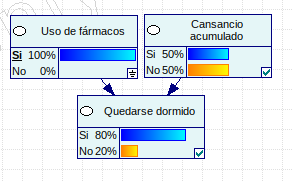
\includegraphics[scale=0.5]{OR2.png}
\end{center}

\begin{center}
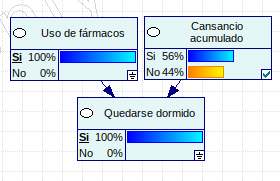
\includegraphics[scale=0.5]{OR3.png}
\end{center}

Como se comprueba, el valor del otro nodo padre, varía al cambiar tamién el valor del nodo hijo, pero no por el cambio del primer nodo padre.\\

\textbf{Modificamos el nodo hijo y uno de los nodos padres}

\begin{center}
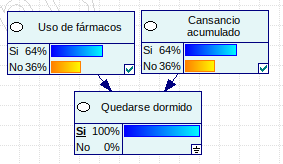
\includegraphics[scale=0.5]{OR4.png}
\end{center}

\begin{center}
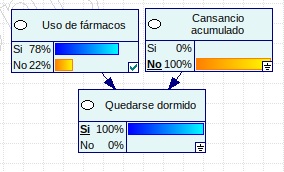
\includegraphics[scale=0.5]{OR5.png}
\end{center}

Como se comprueba, el valor del otro nodo padre, varía al cambiar tamién el valor del nodo padre.\\

\textbf{Efecto \textit{explaining-away}}

En el caso del modelo AND, se puede ver que la probabilidad del otro nodo padre disminuye, mientras que en el caso del modelo OR, la probabilidad aumenta.

\subsection{\textbf{Cabeza-con-cola}}

\textbf{Modelo inicial}

\begin{center}
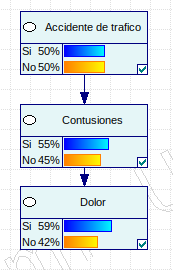
\includegraphics[scale=0.5]{1c1.png}
\end{center}

\textbf{Instanciamos el nodo padre}

\begin{center}
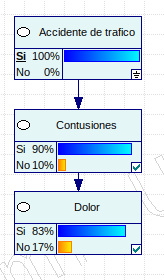
\includegraphics[scale=0.5]{1c2.png}
\end{center}

Y cambiamos el valor del nodo hijo final:

\begin{center}
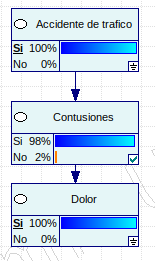
\includegraphics[scale=0.5]{1c3.png}
\end{center}

Podemos ver que el valor de un nodo hijo final afecta al nodo intermedio. Sin embargo, si inicializamos primero el intermedio, cambiar el nodo padre no afecta al hijo final.

\begin{center}
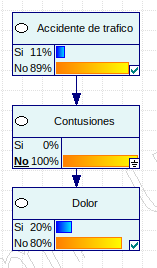
\includegraphics[scale=0.5]{1c4.png}
\end{center}

\begin{center}
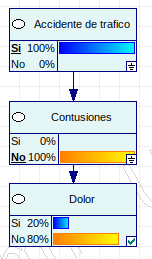
\includegraphics[scale=0.5]{1c5.png}
\end{center}

\section{\textbf{Ejercicio 2}}

Razonamiento en el problema de clasificación del planeta Zyx. Para el problema del
planeta Zyx, razona cómo clasificarías a los siguientes animales:

\begin{enumerate}[label=\alph*)]
\item Un animal rojizo que cojea
\item Un animal de piel escamosa que no cojea
\item Un animal de cinco patas con piel suave
\end{enumerate}

\newpage

\subsection{Solución}

\begin{enumerate}[label=\alph*)]
\item Un animal rojizo que cojea
\begin{center}
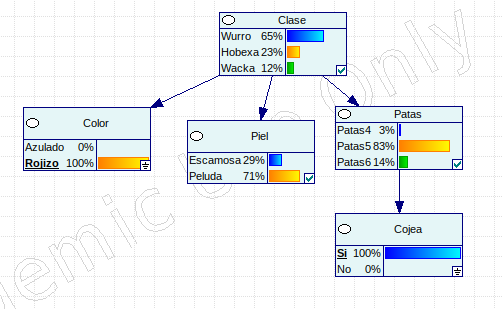
\includegraphics[scale=0.5]{2a.png}
\end{center}
\item Un animal de piel escamosa que no cojea
\begin{center}
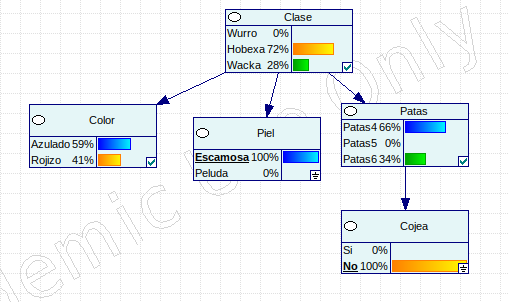
\includegraphics[scale=0.5]{2b.png}
\end{center}
\newpage
\item Un animal de cinco patas con piel suave
\begin{center}
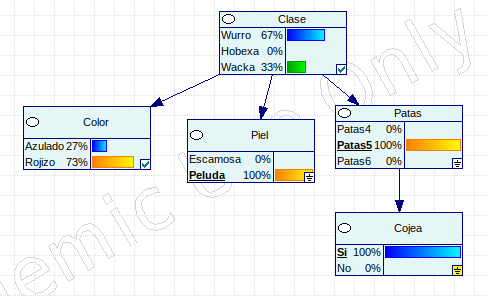
\includegraphics[scale=0.5]{2c.png}
\end{center}
\end{enumerate}

\section{\textbf{Ejercicio 3}}

En el problema de Luis y su alergia a los gatos, explica la evolución de las
probabilidades bajo los siguientes supuestos previos:

\begin{itemize}[label={}]
  \item \textbf{Supuesto 1.} Luis \textbf{no} es alérgico a los gatos
  
  \textit{Nota: En este supuesto, la evidencia 1 sería “Luis no es alérgico a los gatos”, la evidencia 2 sería “Luis estornuda” y la evidencia 3 sería “Los muebles están arañados”}
  \item \textbf{Supuesto 2.} Luis \textbf{es} alérgico a los gatos
  
  \textit{Nota: En este supuesto, la evidencia 1 sería “Luis es alérgico a los gatos”, la evidencia 2 sería “Luis estornuda” y la evidencia 3 sería “Los muebles están arañados”}
\end{itemize}

\newpage

\subsection{Solución}

\begin{itemize}[label={}]
  \item \textbf{Supuesto 1.} Luis \textbf{no} es alérgico a los gatos
 	\begin{center}
	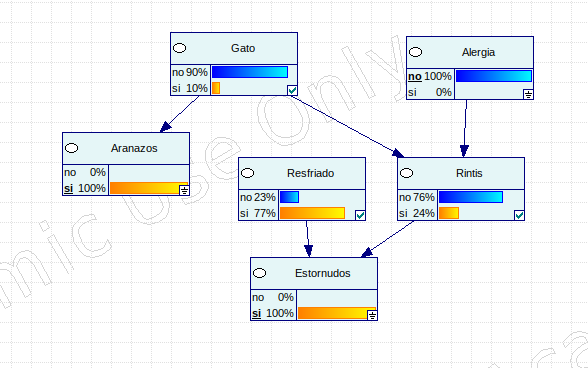
\includegraphics[scale=0.5]{3a.png}
	\end{center}
  \item \textbf{Supuesto 2.} Luis \textbf{es} alérgico a los gatos
	\begin{center}
	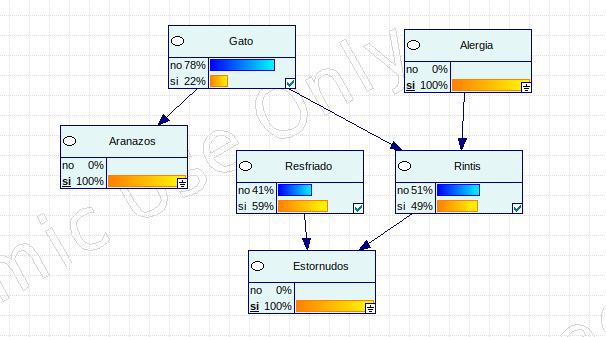
\includegraphics[scale=0.5]{3b.png}
	\end{center}
\end{itemize}

\section{\textbf{Ejercicio Opcional}}

Supongamos de nuevo el planeta Zyx (ejercicio 2). Las Hobexas y Wackas son confiadas e
inofensivas. La escamosa piel de las Hobexas es muy apreciada, por lo que cada piel se vende por 6000 euros. La piel de las Wackas se vende por 4000 euros. Los Wurros no solamente son
imposibles de capturar, sino que se defienden a coces, causando daños por valor de 2000 euros. Razona si merecería la pena económicamente intentar capturar a los animales de los apartados a), b) y c).

Este problema que has resuelto en este apartado se puede implementar en GeNIe a través de las
llamadas “Decision Networks” (redes de decisión). Investiga en el manual cómo se implementan
dichos modelos, y crea uno para este problema. Comprueba que los resultados que has dado en
el apartado anterior son correctos. 

\subsection{Solución}

\textbf{Primer apartado}

\begin{center}
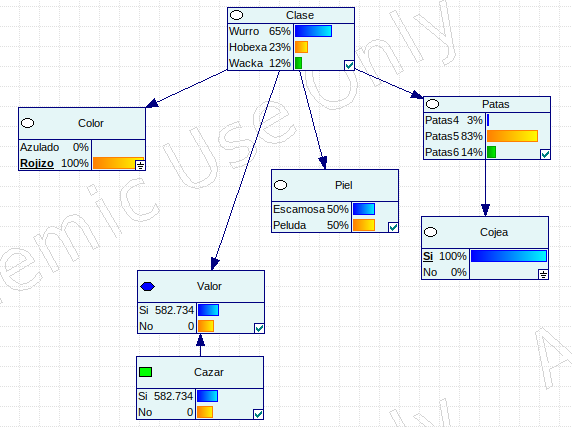
\includegraphics[scale=0.5]{a.png}
\end{center}

\newpage

\textbf{Segundo apartado}

\begin{center}
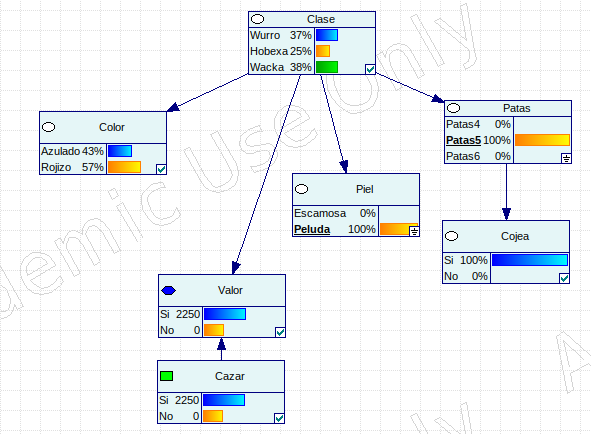
\includegraphics[scale=0.5]{b.png}
\end{center}

\textbf{Tercer apartado}

\begin{center}
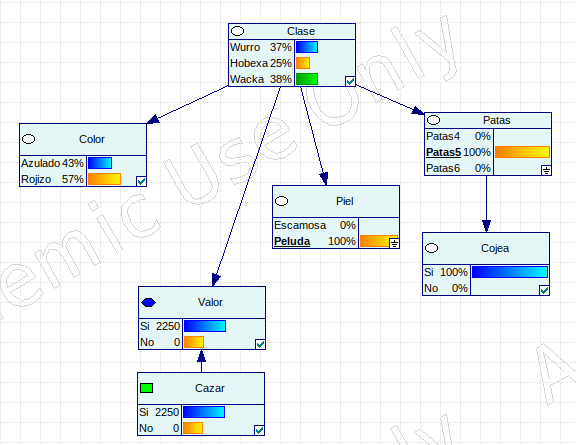
\includegraphics[scale=0.5]{c.png}
\end{center}

Con estos datos, vemos que obtendríamos mayores beneficios si vieramos a una criatura como la del apartado b), es decir, a un animal con piel escamosa que no cojea.

\begin{thebibliography}{9}
\bibitem{Bayes} Información oficial de GeNIe, \url{https://www.bayesfusion.com}.
\end{thebibliography}

\end{document}